\providecommand{\main}{../../..}
\documentclass[\main/main.tex]{subfiles}
\begin{document}

\subsection{Exercise 15}
The following decision problem is given, with 3 alternatives and 2 attributes (utilities), having weights $\w$:

\begin{table}
  \begin{tabular}{L|LLL}
    \text{Attributes} & A  & B  & C  \\
    \hline
    u_1               & 80 & 20 & 60 \\
    u_2               & 10 & 90 & 50
  \end{tabular}
  \begin{tabular}{L|L}
         & \text{Weights} \\
    \hline
    \w_1 & 0.7            \\
    \w_2 & 0.3
  \end{tabular}
\end{table}

Determine the best alternative with the method of the weighted sum.

Carry out a sensitivity analysis on the weight $\w_1$.

\subsection{Exercise 15 resolution}

\subsubsection*{Weighted sum}

\begin{table}
  \begin{tabular}{L|LLL}
    \text{Attributes} & A  & B  & C  \\
    \hline
    u^*               & 59 & 41 & 57 \\
  \end{tabular}
\end{table}

The method of the weighted sum suggests $A$ as the optimal solution.

\subsubsection*{Sensitivity analysis}
Using $\w_1$ as our knob, we define $\w_2$ as $\w_2 = 1-\w_1$.

\begin{figure}
  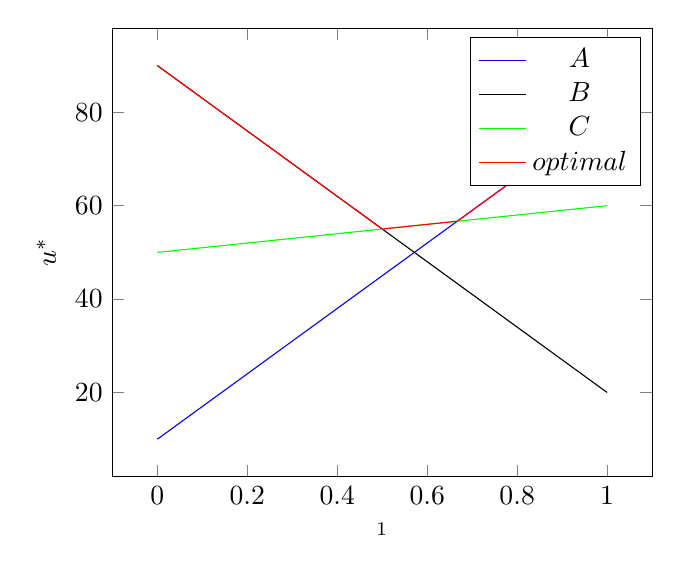
\begin{tikzpicture}
    \begin{axis}[
        xlabel=$\w_1$,
        ylabel=$u^*$,
        domain=0:1
      ]
      \addplot[mark=none,color=blue]{
        80*x+10*(1-x)
      };
      \addplot[mark=none,color=black]{
        20*x+90*(1-x)
      };
      \addplot[mark=none,color=green]{
        60*x+50*(1-x)
      };
      \addplot[mark=none,color=red]{
        max(max(
        60*x+50*(1-x),
        80*x+10*(1-x)
        ),
        20*x+90*(1-x)
        )
      };
      \legend{$A$, $B$, $C$, $optimal$}
    \end{axis}
  \end{tikzpicture}
  \caption{The solution $A$ remains optimal for $\w_1 \geq \frac{2}{3} = 0.6\bar{6}$}
\end{figure}

\end{document}